\usetikzlibrary{angles,quotes,decorations.pathreplacing}
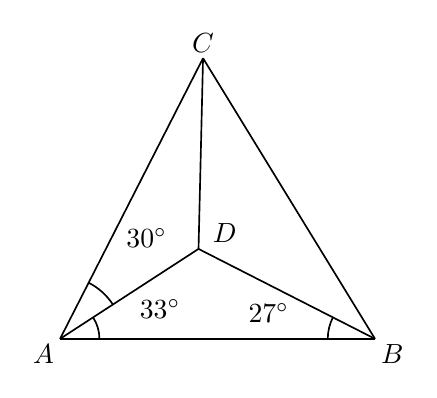
\begin{tikzpicture}[x=1cm,y=1cm,font=\normalsize,
 geometry edge/.style={solid,line width=.6pt},
 geometry mark/.style={solid,line width=.6pt},
 geometry label/.style={font=\normalsize,inner sep=2pt}]
\coordinate (A) at (0.0,0.0);
\coordinate (B) at (4.0,0.0);
\coordinate (C) at (1.815961999,3.564026097);
\coordinate (D) at (1.758601854,1.142049398);
\coordinate (LA30) at (1.100000000,1.280000000);
\coordinate (LA33) at (1.270000000,0.375000000);
\coordinate (LB27) at (2.650000000,0.330000000);
\draw[geometry edge] (A)--(B);
\draw[geometry edge] (B)--(C);
\draw[geometry edge] (C)--(A);
\draw[geometry edge] (A)--(D);
\draw[geometry edge] (B)--(D);
\draw[geometry edge] (C)--(D);
\pic[draw, geometry mark, angle radius=5mm] {angle=B--A--D};
\pic[draw, geometry mark, angle radius=8mm] {angle=D--A--C};
\pic[draw, geometry mark, angle radius=6mm] {angle=D--B--A};
\node[geometry label,below left] at (A) {$A$};
\node[geometry label,below right] at (B) {$B$};
\node[geometry label,above] at (C) {$C$};
\node[geometry label,above right,xshift=3pt] at (D) {$D$};
\node[geometry label] at (LA30) {$30^\circ$};
\node[geometry label] at (LA33) {$33^\circ$};
\node[geometry label] at (LB27) {$27^\circ$};
\end{tikzpicture}
